% how to compile: $ pdflatex row-column-vertices-grid.tex && pdf2svg row-column-vertices-grid.pdf row-column-vertices-grid.svg
\documentclass[tikz]{standalone}

\begin{document}
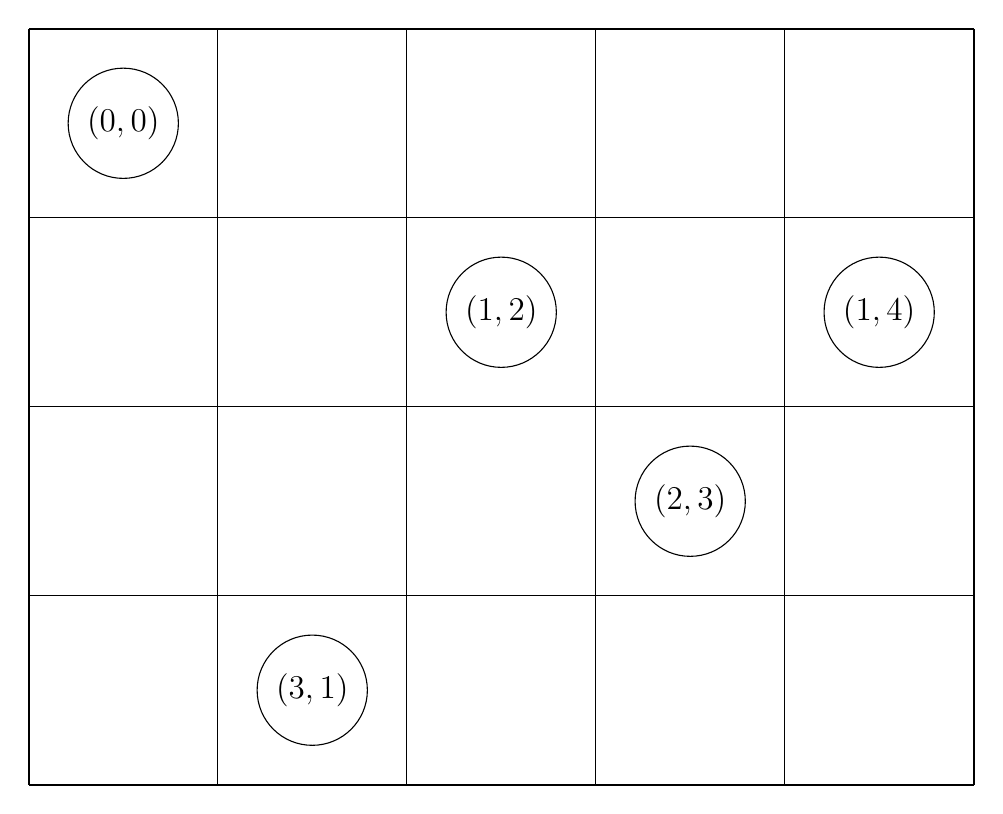
\begin{tikzpicture}[
    x=2.4cm,
    y=-2.4cm,
    font=\large,
]
    % \path[fill, color=white] (0, 0) rectangle (5, 4);
    \path[draw, thick] (0, 0) -- (5, 0);
    \path[draw] (0, 1) -- (5, 1);
    \path[draw] (0, 2) -- (5, 2);
    \path[draw] (0, 3) -- (5, 3);
    \path[draw, thick] (0, 4) -- (5, 4);
    \path[draw, thick] (0, 0) -- (0, 4);
    \path[draw] (1, 0) -- (1, 4);
    \path[draw] (2, 0) -- (2, 4);
    \path[draw] (3, 0) -- (3, 4);
    \path[draw] (4, 0) -- (4, 4);
    \path[draw, thick] (5, 0) -- (5, 4);

    \node[draw, circle, fill=white, minimum size=1.4cm] (c00) at (0.5, 0.5) {$(0, 0)$};
    \node[draw, circle, fill=white, minimum size=1.4cm] (c21) at (2.5, 1.5) {$(1, 2)$};
    \node[draw, circle, fill=white, minimum size=1.4cm] (c41) at (4.5, 1.5) {$(1, 4)$};
    \node[draw, circle, fill=white, minimum size=1.4cm] (c32) at (3.5, 2.5) {$(2, 3)$};
    \node[draw, circle, fill=white, minimum size=1.4cm] (c13) at (1.5, 3.5) {$(3, 1)$};
\end{tikzpicture}
\end{document}
